% Math symbols and examples: http://en.wikibooks.org/wiki/LaTeX/Mathematics
% Also useful link: http://en.wikibooks.org/wiki/LaTeX/Advanced_Mathematics

% This document is used for title generating of exercise solutions. 
% Also it used for generating styles and environmentof documents.
% To add this title in document add next line:
% % This document is used for title generating of exercise solutions. 
% Also it used for generating styles and environmentof documents.
% To add this title in document add next line:
% % This document is used for title generating of exercise solutions. 
% Also it used for generating styles and environmentof documents.
% To add this title in document add next line:
% \input{../template.tex}
\documentclass[a4paper]{article}
\usepackage[utf8]{inputenc}
\usepackage[top=1.5cm]{geometry}
\usepackage{amssymb}
\usepackage{enumitem}
\usepackage{amsmath}

\allowdisplaybreaks

\DeclareMathOperator{\ggT}{ggT}
\DeclareMathOperator{\kgV}{kgV}

\title{Mathematik: Diskrete Strukturen \\ \Large Lösungsblatt}
\author{Anton Bubnov, Eugen Kuzmenko}

\documentclass[a4paper]{article}
\usepackage[utf8]{inputenc}
\usepackage[top=1.5cm]{geometry}
\usepackage{amssymb}
\usepackage{enumitem}
\usepackage{amsmath}

\allowdisplaybreaks

\DeclareMathOperator{\ggT}{ggT}
\DeclareMathOperator{\kgV}{kgV}

\title{Mathematik: Diskrete Strukturen \\ \Large Lösungsblatt}
\author{Anton Bubnov, Eugen Kuzmenko}

\documentclass[a4paper]{article}
\usepackage[utf8]{inputenc}
\usepackage[top=1.5cm]{geometry}
\usepackage{amssymb}
\usepackage{enumitem}
\usepackage{amsmath}

\allowdisplaybreaks

\DeclareMathOperator{\ggT}{ggT}
\DeclareMathOperator{\kgV}{kgV}

\title{Mathematik: Diskrete Strukturen \\ \Large Lösungsblatt}
\author{Anton Bubnov, Eugen Kuzmenko}


\begin{document}
    \maketitle
    \section*{Vertiefung:}
    \begin{enumerate}[label=(\alph*)]
        % Task (a)
        \item  Ein ebener,
        k-regulärer Graph besteht aus
        12 Knoten und teilt die Ebene in
        14 Gebiete. Wie groß ist k? \\
        Nach Theorem 3.23 gilt $||F|| = ||E|| - ||V|| + 2$. Für unseren Fall bedeutet das also:
        $14 = ||E|| - 12 + 2 \implies E = 24$ \\
        Des weiteren gilt nach Proposition 3.3: \\
        $\sum_{v \in V} deg(v) = 2 \cdot ||E||$. D.h. die Summe der Grade ist $2 * 24 = 58$. \\
        Daraus folgt $\frac{58}{12} = 4 = k$
        
        %Task (b)
        \item Task b
        
        %Task c
        
        \item Task c
        %Task d
        
        \item Ist der $Q_3$ planar? 
        Ja. Betrachte dazu folgende Graphik:\\
        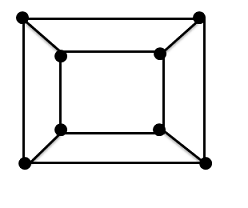
\includegraphics{Q3}
        
        %Task e
        \item Ist der $Q_4$ planar?
        Nein. Der $Q_4$ enthält einen $K_{3,3}$ als Teilgraphen. wenn man diesen Teilgraphen "aufspannt" gibt es Überkreuzungen im gesamten Graphen. Daraus folgt, dass der $Q_4$ nicht planar sein kann.
        %Task f
        \item
        
        % Task g
        \item
        
        % Task h
        \item
        % Task i
        \item Wie viele Knotenfärbungen mit k Farben hat ein $K_n$ ?
        Da jeder Knoten n-1 Nachbarn hat (jeder Knoten ist mit jedem verbunden) hat der $K_n n$ Farben. Den ersten Knoten kann beliebig wählen, weshalb es $k$ Möglichkeiten zur Färbung gibt. Für die weiteren Knoten gibt es immer eine Möglichkeit weniger, für eine Färbung. Folglich gibt es: \\
        $\prod_{i=0}^{k-1} k - i = i^k $ Möglichkeiten zur Färbung eines $K_n$
          
        % Task j
        \item
        
    \end{enumerate}
    \section*{Kreativität:}
    \begin{enumerate}[label=(\alph*)]
    	%Task (a)
    	\item Task a
    \end{enumerate}
    \section*{Transfer:}
    \begin{enumerate}[label=(\alph*)]
    	\item Task a
    \end{enumerate}
\end{document}






